% Autor: Lukas Deeken
% Letzte Bearbeitung: 01.05.2022

\chapter{Mechanische Systeme}
An dieser Stelle geht mein Dank an Florian Irle, der obwohl er sich eigentlich etwas aus dem Projekt zurückhalten wollte, mit einem beispiellosen Tatendrang an der Entwicklung und Konstruktion des Antriebssysteme besonders des Getriebegehäuses und des Gussprozesses mitgearbeitet hat.

%\section{Antriebslayout}
%
%2WD ein motor (diff)
%2Wd zwei motor (gewähltes konzept, Torque vektoring/hinterachslenkung)
%4WD (Komplexität ungefederte massen etc.)
%
%kurz was gibt es und warum machen wir das was wir machen
%referenz zu vorher erstellten Dokumenten
%
%\section{Packaging}
%Packaging leistungskennzahl. Volumenfüllungsgrad, schwerpunkt position, wartungsaufwand
%CAD Stuff benötigt

%\section{Systeme}

\section{Kühlung}

\begin{figure}[H]
	\centering
	
\usetikzlibrary{arrows}
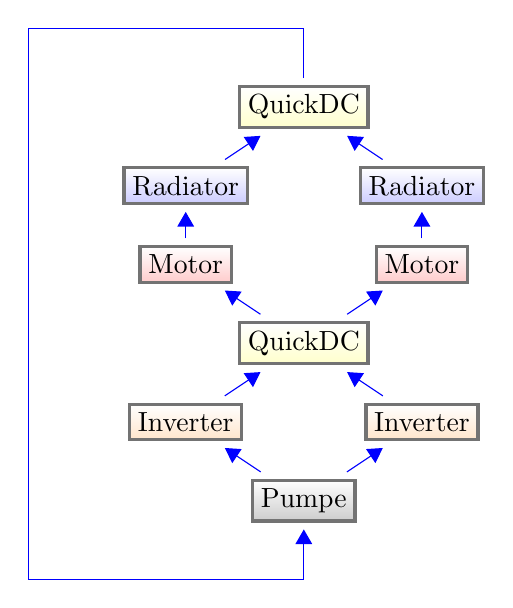
\begin{tikzpicture}
\tikzstyle{radiator} = [draw,outer sep=3,inner sep=3,line width=1, very thick, draw=black!55, top color=white,bottom color=blue!20]
\tikzstyle{Pumpe} = [draw,outer sep=3,inner sep=3,line width=1, very thick, draw=black!55, top color=white,bottom color=black!20]
\tikzstyle{Inverter} = [draw,outer sep=3,inner sep=3,line width=1, very thick, draw=black!55, top color=white,bottom color=orange!20]
\tikzstyle{Motor} = [draw,outer sep=3,inner sep=3,line width=1, very thick, draw=black!55, top color=white,bottom color=red!20]
\tikzstyle{Quickconnect} = [draw,outer sep=3,inner sep=3,line width=1, very thick, draw=black!55, top color=white,bottom color=yellow!20]

\node [radiator] (v7) at (-2,-2.5) {Radiator};
\node [radiator] (v8) at (1,-2.5) {Radiator};
\node [Pumpe] (v1) at (-0.5,-6.5) {Pumpe};
\node [Inverter] (v2) at (-2,-5.5) {Inverter};
\node [Inverter] (v3) at (1,-5.5) {Inverter};
\node [Motor] (v6) at (-2,-3.5) {Motor};
\node [Motor] (v5) at (1,-3.5) {Motor};
\node [Quickconnect] (v4) at (-0.5,-4.5) {QuickDC};
\node [Quickconnect] (v9) at (-0.5,-1.5) {QuickDC};

\tikzstyle{Leitungen} = [-triangle 60, color=blue]
\draw [Leitungen] (v1) edge (v2);
\draw [Leitungen] (v1) edge (v3);
\draw [Leitungen] (v2) edge (v4);
\draw [Leitungen] (v3) edge (v4);
\draw [Leitungen] (v4) edge (v5);
\draw [Leitungen] (v4) edge (v6);
\draw [Leitungen] (v6) edge (v7);
\draw [Leitungen] (v5) edge (v8);
\draw [Leitungen] (v7) edge (v9);
\draw [Leitungen] (v8) edge (v9);

\draw [Leitungen] (v9) -- (-0.5,-0.5) -- (-4,-0.5) -- (-4,-7.5) -- (-0.5,-7.5) -- (v1);
\end{tikzpicture}
	\caption{Kühlsystem Übersicht}
	\label{abb:Coolingssystem}
\end{figure}

\FloatBarrier
\subsection{Radiator}
Die Berechnung des Radiators basiert auf der Annahme das hier eine Ähnlichkeitstheorie Anwendung finden kann. Hierbei wurden die bekannten realen (index r) Eingangsparameter aus Messungen am Vorjahresfahrzeug mit den Modellparametern (index m) für das kommende Fahrzeug in Beziehung gesetzt. Konkret die Temperaturdifferenz am Eintritt und der Wärmestrom. Hierbei wurde kein klassischer Weg bekannt aus der Thermodynamik über NTU-Schaubilder etc. gewählt da die geometrischen Parameter des Radiators abgesehen von der frontalen Netzfläche nicht bekannt waren. Zur genaueren Betrachtung sollte dieses Vorgehen in Zukunft vergleichend angewendet werden. Folgend die angewendete Formel.

\begin{equation}
		\label{eqn:KühlerÄhnlichkeitsformel}
		\dfrac {\glsc{symb:A_r}} {\glsc{symb:A_m}} = \dfrac {\glsc{symb:Qdot_r} * \glsc{symb:deltaT_ein r}} {\glsc{symb:Qdot_m} * \glsc{symb:deltaT_ein m}}
\end{equation}

Sie besagt, dass das Verhältnis der Kühlerflächen proportional zu dem Verhältnis von Wärmestrom und Eingangstemperaturdifferenz ist.\\
\\
Hierbei ist \glsc{symb:A_r} vom Vorjahresfahrzeug bekannt, \glsc{symb:Qdot_r} ergibt sich mit folgender Formel aus den Vor- und Rück/-lauftemperaturen vom Wärmetauscher sowie dem Wassermassenstrom welche beim TY19 gemessen wurden.

\begin{equation}
	\glsc{symb:Qdot_r} = \glsc{symb:Cv_wasser} * \glsc{symb:Vdot_wasser} * \glsc{symb:rho_wasser} * (\gls{symb:t_ein Wasser} - \glsc{symb:t_aus Wasser}) * Anzahl\textsubscript{Kühler}
\end{equation}

\glsc{symb:Qdot_m} wird mit Hilfe der \ac{LTS} ermittelt. Hier werden sämtlich Verluste die in das Kühlsystem eingetragen werden im Rahmen der Rundenzeitberechnung über den Endurance Fahrtzyklus gemittelt mit gerechnet.\\
\\
\glsc{symb:deltaT_ein m} wird mit \ensuremath{30 K} angenommen. Die max. Temperatur des Kühlwassers sollte \ensuremath{60°C} nicht überschreiten währen im Hochsommer mit Umgebungstemperaturen von \ensuremath{30°C} zu rechnen ist.\\
\\
Mit der Formel \ref{eqn:KühlerÄhnlichkeitsformel} umgestellt nach \glsc{symb:A_m} kann nun die Kühlerfläche für das Elektrofahrzeug bestimmt werden.

\begin{equation}
	\glsc{symb:A_m} = \dfrac {\glsc{symb:A_r} * \glsc{symb:Qdot_m} * \glsc{symb:deltaT_ein m}} {\glsc{symb:Qdot_r} * \glsc{symb:deltaT_ein r}}
\end{equation}

Dies führt zu folgenden Ergebnissen.

\begin{table}[h]
	\centering
	\begin{tabular}{|c|c|c|}
		\hline
		\multicolumn{3}{|c|}{Eingangsparameter} \\
		\hline
		\glsc{symb:A_r} & 0,099 & \ensuremath{m^2} \\
		\hline
		\glsc{symb:t_ein Wasser} & 73,16 & °C \\
		\hline
		\glsc{symb:t_aus Wasser} & 70,37 & °C \\
		\hline
		\glsc{symb:rho_wasser} & 997 & \ensuremath{Kg/m^3} \\
		\hline
		\glsc{symb:Vdot_wasser} & 36,26 & \ensuremath{l/min} \\
		\hline
		\glsc{symb:Cv_wasser} & 4190 & \ensuremath{J/Kg K} \\
		\hline
		\glsc{symb:deltaT_ein r} & 43,16 & \ensuremath{K} \\
		\hline
		\glsc{symb:deltaT_ein m} & 30 & \ensuremath{K} \\
		\hline
		\glsc{symb:Qdot_m} & 5364 & \ensuremath{W} \\
		\hline
		\multicolumn{3}{|c|}{Ergebnisse} \\
		\hline
		\glsc{symb:Qdot_r} & 14089 & \ensuremath{W} \\
		\hline
		\glsc{symb:A_m} & 0,026 & \ensuremath{Kg/s} \\
		\hline
	\end{tabular}
\end{table}

Dies ergibt mit unserem Modell eine Reduktion auf \ensuremath{26,46 \%} der vorherigen Kühlerfläche. Die Baugröße die am ende für den Kühler gewählt wurde entspricht ca. \ensuremath{50 \%} der Kühlerfläche also das doppelte vom Rechenergebnis. Eine derart hohe Sicherheit ist darauf zurückzuführen das die Berechnung von Wärmeübertragern generell keine sehr exakte Wissenschaft ist und der Bauraum eine derartige Überdimensionierung an der Stelle zugelassen hat.\\

\FloatBarrier
\subsection{Lüfter}
Für die Auslegung des Lüfters wurde von der Aerodynamik Abteilung vorgegeben das man die Abluft des Systems nutzen möchte um das Strömungsprofil am Diffusor zu beeinflussen. Hierfür mussten Strömungsgeschwindigkeiten im Bereich der \ensuremath{80-90 km/h} am Auslass erreicht werden. Für den Lüfter wurde auch in den letzten Jahren am Verbrenner ein Drohnennmotor mit Propeller und externer Ansteuerung verwendet, da dies deutlich leichter ist als eine fertige Einheit. In diesem Zuge sollten Volumenstrom und Ausgangsgeschwindigkeiten für verschiedene Konzepte berechnet werden können. Aufgrund der Größe des Kühlers kamen nur \ensuremath{4 Zoll} oder kleiner Propeller in Frage. Weiterhin ist die Fragestellung aufgekommen ob ein Propeller ausgelegt für Freiströmung sinnvoll vor einem Lamellen-Kreuzstrom-Wärmeübertrager einzusetzen ist. Hierfür wurde zum Vergleich ein Lüfter von der Firma EBM-Papst \cite{3214JH4Datenblatt} beschafft um die Leistungsdaten schlussendlich vergleichen zu können.\\
\\
Für Drohnenmotoren sind in der Regel Daten für Schubkraft und Leistung verfügbar. Dies Lässt sich mit Hilfe des 2. Newtonschen Gesetztes, dem Impulssatz, umrechnen. Wir nehmen dabei an das unser Fahrzeug still steht. Dies führt zu folgender Gleichung.

\begin{equation}
	\glsc{symb:F_Schub} = \glsc{symb:mdot_Luft} * \glsc{symb:v_Luft}
\end{equation}

Dies lässt sich mit folgenden Formeln Umstellen.

\begin{equation}
	\glsc{symb:mdot_Luft} = \glsc{symb:Vdot_Luft} * \glsc{symb:rho_Luft}
\end{equation}
\begin{equation}
	\glsc{symb:Vdot_Luft} = \glsc{symb:A_Prop} * \glsc{symb:v_Luft}
\end{equation}

Und führt zu.

\begin{equation}
	\glsc{symb:v_Luft} = \sqrt{\dfrac{\glsc{symb:F_Schub}} {\glsc{symb:A_Prop} * \glsc{symb:rho_Luft}}}
\end{equation}

Mit diesen Gleichungen können wir auch den Volumen- und Massenstrom bestimmen.\\
\\
Mit folgender Formel lässt sich die Luftleistung bestimmen.

\begin{equation}
	\glsc{symb:P_Luft} = \dfrac{\glsc{symb:mdot_Luft}}{2} * \glsc{symb:v_Luft}^2
\end{equation}

Damit können wir schlussendlich die Effizienz des Design beurteilen.

\begin{equation}
	\glsc{symb:eta_Luefter} = \dfrac{\glsc{symb:P_Luft}}{\glsc{symb:P_elektrisch}}
\end{equation}

Entschieden wurde sich am ende für den T-Motor F2004-1700KV zusammen mit dem Gemfan 4023 Propeller. Daten dafür in folgender Tabelle.

\begin{table}[h]
\centering
\begin{tabular}{|c|c|c|}
	\hline
	\multicolumn{3}{|c|}{Eingangsparameter} \\
	\hline
	\glsc{symb:A_Prop} & 8107 & \ensuremath{mm^2} \\
	\hline
	\glsc{symb:F_Schub} & 650 & g \\
	\hline
	\glsc{symb:P_elektrisch} & 286 & W \\
	\hline
	\glsc{symb:rho_Luft} & 1,225 & \ensuremath{Kg/m^3} \\
	\hline
	\multicolumn{3}{|c|}{Ergebnisse} \\
	\hline
	\glsc{symb:v_Luft} & 25,339 & \ensuremath{m/s} \\
	\hline
	\glsc{symb:mdot_Luft} & 0,25 & \ensuremath{Kg/s} \\
	\hline
	\glsc{symb:Vdot_Luft} & 0,21 & \ensuremath{m^3/s} \\
	\hline
	\glsc{symb:P_Luft} & 80,79 & W \\
	\hline
	\glsc{symb:eta_Luefter} & 28 & \% \\
	\hline
\end{tabular}
\end{table}

Im Rahmen der Systembetrachtung wurden am tatsächlichen Aufbau einige Messdaten genommen.

\begin{table}[h]
	\centering
	\begin{tabular}{|c|c|c|}
		\hline
		\multicolumn{3}{|c|}{T-Motor F2004} \\
		\hline
		\glsc{symb:v_Luft} & 75 & \ensuremath{km/h} \\
		\hline
		\glsc{symb:P_elektrisch} & 195 & \ensuremath{W} \\
		\hline
		\multicolumn{3}{|c|}{EBM Papst 3214jh4} \\
		\hline
		\glsc{symb:v_Luft} & 73 & \ensuremath{km/h} \\
		\hline
		\glsc{symb:P_elektrisch} & 50 & \ensuremath{W} \\
		\hline
	\end{tabular}
\end{table}

Mit Hilfe der Vorherigen Rechnung können wir nun den gleichen Rechenweg Rückwärts gehen um uns wieder alle übrigen Parameter zu berechnen. Die Lüftausströmfläche beträgt dabei \ensuremath{0,004173m^2}.

\begin{table}[h]
	\centering
	\begin{tabular}{|c|c|c|}
		\hline
		\multicolumn{3}{|c|}{T-Motor F2004} \\
		\hline
		\glsc{symb:v_Luft} & 75 & \ensuremath{km/h} \\
		\hline		
		\glsc{symb:Vdot_Luft} & 0,087 & \ensuremath{m^3/s} \\
		\hline
		\glsc{symb:mdot_Luft} & 0,107 & \ensuremath{kg/s} \\
		\hline
		\glsc{symb:P_Luft} & 23,115 & \ensuremath{W} \\
		\hline
		\glsc{symb:eta_Luefter} & 12 & \ensuremath{\%} \\
		\hline		
		\multicolumn{3}{|c|}{EBM Papst 3214jh4} \\
		\hline
		\glsc{symb:v_Luft} & 75 & \ensuremath{km/h} \\
		\hline
		\glsc{symb:Vdot_Luft} & 0,085 & \ensuremath{m^3/s} \\
		\hline
		\glsc{symb:mdot_Luft} & 0,104 & \ensuremath{kg/s} \\
		\hline
		\glsc{symb:P_Luft} & 21,315 & \ensuremath{W} \\
		\hline
		\glsc{symb:eta_Luefter} & 43 & \ensuremath{\%} \\
		\hline		
	\end{tabular}
\end{table}

Laut EBM Papst liegen die zu erwartende Effizienzen bei einem Axialgebläse im Bereich von \ensuremath{25\% - 65\%}. Daran ist zu erkennen das unser aktueller Lüfter von EBM noch nicht die effizienteste Lösungen darstellt und unser Drohnenmotor eine sehr ineffiziente Lösung ist. Dennoch ein Aufbau mit Lüftern von EBM wiegt ca. \ensuremath{560 g} während der Aufbau mit Drohnennmotoren bei ca. \ensuremath{55 g} liegt. Allein diese Gewichtsersparnis ist den Einsatz dieses Gebläses wert. Empfehlenswert wäre an der Stelle die Optimierung des Rotorblattes auf den vorliegenden Anwendungsfall.

\FloatBarrier
\subsection{Wasserpumpe und Schläuche}

Für die Auslegung des Wasserkreislaufes sind die Druckabfälle der Einzelsysteme relevant, zur Referenz die Systemübersicht \ref{abb:Coolingssystem}\\
\\
Des weiteren sind für die Betrachtung weitere Parameter relevant. Laut Motorhersteller \cite{ManualEmrax208} liegt der optimale Wasservolumenstrom bei  \ensuremath{6-8l/min}. Aus der Vorhergehenden Betrachtung geht hervor das die umzusetzende Wärmeleistung bei \ensuremath{5364 W} liegt. Der angepeilte Luftvolumenstrom durch einen Kühler beläuft sich auf \ensuremath{756 m^3/h}.\\
\\
Mit den folgenden beiden Diagrammen \ref{fig:elwleistung-uber-volumenstrom} und \ref{fig:elw-druckabfall-uber-volumenstrom} aus dem Leistungsdatenblatt für die ELW-Serie, einem in der Bauart ähnlichen Wärmeübertrager, lässt sich der Druckabfall über den Radiator bestimmen.

\begin{figure}[h]
	\centering
	\includegraphics[width=0.7\linewidth]{"bilder/ELW_Leistung über Volumenstrom"}
	\caption{ELW-Leistung über Volumenstrom \cite{DatenblattELW}}
	\label{fig:elwleistung-uber-volumenstrom}
\end{figure}

Unser angestrebter Radiator entspricht mit seiner Netzfläche am ehesten dem ELW3. Dies würde bei den bisher bekannten Betriebsdaten zu eine Kühlleistung von \ensuremath{90 W/K} oder auch \ensuremath{2700 W} führen. Oder bei zwei Einheiten zu \ensuremath{5400 W}. Dies ist sehr nah an der angestrebten Wärmeleistung.

\begin{figure}[h]
	\centering
	\includegraphics[width=0.7\linewidth]{"bilder/ELW-Druckabfall über Volumenstrom"}
	\caption{ELW-Druckabfall über Volumenstrom \cite{DatenblattELW}}
	\label{fig:elw-druckabfall-uber-volumenstrom}
\end{figure}

Die Grafik \ref{fig:elw-druckabfall-uber-volumenstrom} ist an dieser Stelle etwas verwirrend da der ELW 2 und der ELW3 die Farben getauscht hat. Da es sich hierbei jedoch um die einzigen Daten handelt die aufgetrieben werden konnten wird an dieser Stelle angenommen das die grüne Linie für den ELW3 steht und die Lila Linie den ELW 2 darstellt. Dies ist die sichere Annahme, da dies im zweifel zu einem zu hohen Druckabfall und damit einer Überdimensionierung der Anlage führt.\\
Anhand dieser Grafik kann also nun der Druckabfall zu einem entsprechenden Wasservolumenstrom abgelesen werden.\\
\\
Für den Umrichter gibt es im Datenblatt ein fertiges Diagramm, siehe \ref{fig:cooling-characteristik}.
\begin{figure}[h]
	\centering
	\includegraphics[width=0.7\linewidth]{"bilder/Druckabfall DTI500LC"}
	\caption{Druckabfall DTI 500 \cite{manualHV500}}
	\label{fig:cooling-characteristik}
\end{figure}

Für den Motor existieren nur Daten an einem einzigen Punkt. An den anderen Graphen ist jedoch in der Regel ein quadratischer Verlauf zu erkennen, weswegen hier quadratisch regressiert wurde. Wir beginnen mit der allgemeine Formel

\begin{equation}
	Y = A x^2 + B x + C
\end{equation}

Die Linie soll durch den Nullpunkt verlaufen damit wird \ensuremath{C = 0} und wir nehmen an das es keinen linearen Anteil gibt, damit wird \ensuremath{B = 0}. Unsere Gleichung vereinfacht sich zu.

\begin{equation}
	Y = A x^2
\end{equation}

eingesetzt ergibt sich.

\begin{equation}
	0,6 bar = A * (7 l/min)^2  
\end{equation}
\begin{equation}
	A = \dfrac{0,6 bar}{(7 l/min)^2 }
	  = 0,01224 \dfrac{bar}{(l/min)^2}
\end{equation}

Für die Leitungen wurde eine extensive Berechnung durchgeführt, auf die an dieser Stelle leider aus Zeitgründen nicht näher eingegangen werden kann. Die Schlussfolgerung ist jedoch das die Verluste vernachlässigbar klein sind. \\
\\
Die Daten für die Pumpen entstammen direkt den Datenblättern\\
\\
Alle Ergebnisse sind nun in der Systemkennlinie \ref{fig:kuhlsystemkennlinie} abgebildet

\begin{figure}[h]
	\centering
	\includegraphics[width=0.7\linewidth]{bilder/Kühlsystemkennlinie}
	\caption{Kühlsystemkennlinie}
	\label{fig:kuhlsystemkennlinie}
\end{figure}

Der Punkt an dem sich die Linien der jeweiligen Pumpe mit der Linie des Gesamtsystem schneidet ist der Betriebspunkt des Systems. Dieser Druckabfall und dieser Volumenstrom sollten sich im Betrieb einstellen. Bei der Grafik \ref{fig:kuhlsystemkennlinie} muss beachtet werden das dies von der Pumpe aus betrachtet wird und daher der Volumenstrom doppelt so groß ist wie am kühler aufgrund der zwei separaten Kühleinheiten.

\FloatBarrier

%\subsubsection{Outbound vs Inbound}
%Radnabenmotor vs interner motor 
%ungeferte massen
%packaging im rad problem(Planetengetriebe) fertigungsaufwand innenzahnkranz, generell zahnräder
%keine Antriebswellen
%besseres packaging im auto
%
%\subsection{Antrieb} (Michel und Linus)
%Kettentrieb vs Stirnradgetriebe
%	Kettentrieb leichter günstiger, simpler (keine öldichtigkeit von nöten)
%	Getriebe Kompakter, weniger Umschlagspiel (rekuperativbetrieb), weniger wartungsintensiv (kettentrieb hält ca. 6-8h)
%zahnrad auslegung
%	Getriebebeleg (Basics)
%	Soiftware kurz es gibt Sie wie sie heißt und fertig
%Zahnrad fertigung
%	Profilstoßen
%	Profilfräsen (Scheiben odser schaft)
%	Wälzfräsenm
%	Waserstrahlen
%Kettentrieb alternative
%	Auslegung (berechnungen)
%Wellen auslegung
%	Überschalgsrechnung (Getriebebeleg) 
%	Anbindungsmaße (Lager, tripoden, zahräder etc)
%Lagerberechnung
%FEM detour
%	Netzunabhängigkerit
%	konvergenz
%	Kräfte richtig antragen
%	Feste flächen richtig wählen
%	kräfte richtig berechnen
%	Kontaktflächen bestimmen
%	Feinheitsgrade des netz
%	Inventor Casual fixe abschätzung oder einfache probleme vs Ansys Profi tool für komplexe verlässliche analyse
%
%\subsubsection{Gussgehäuse vs Fräsgehäuse vs Schweißgehäuse} (Flo Irle)
%Vor und nachteile
%	Guss günstig
%	Fräsen Einfache auslegung
%	Schweiß einfache fertigung
%	
%
%eingehen aufs gussgehäuse
%
%SES anforderungen
%Flexural rigidity
%E modul vs yield strenght welche verbnesserungen bringen wo was
%Gussimulation
%FEM Bilder
%CAD Bilder
%Formkasten
%Heizofen
%tiegel
%trageschere
%gussmaterial auswahl
%kellen etc. für zusätze
%wärmebehandlung
%materialtests
%zusatzstoffe guss
%stuff von Floh?
%
%\subsubsection{Antriebswellen und Tripoden} Störle und schrang
%excel tabellen und stuff von Störle und schrang
%
%FEM sim bilder von Schrang
